\section{Experimental Results}
\label{sec:result}

This section presents experiment results and answer the RQs by
studying the results quantitatively and qualitatively.

%% \InputWithSpace{tables/test-results-table}
\InputWithSpace{tables/test-results-3-50-table}
\InputWithSpace{tables/test-results-3-100-table}
\InputWithSpace{tables/test-results-3-200-table}

\subsection{RQ1: Test Suite Diversity}

Our experimental results show that \emph{\tool generated many test cases that the sentiment analysis models failed to predict the correct labels, and it produced significantly more diverse test cases than \Cklst did.}

Table~\ref{table:TestResult} shows the testing results of three \sa models. First column lists 
linguistic capabilities for the \sa task, and Columns 2-3 show 
the numbers of seed and expanded test cases, respectively. 
Columns 4-5 show the failure rate (i.e., percentage of test cases that a model predicts incorrect label) of each \sa models on the seed and expanded test cases respectively. 
Column 6 shows the number of expanded test cases that failed,
but their corresponding seed test cases passed.

We observe that in all but one linguistic capabilities,
\tool produces hundreds of test cases, expanding at least an order of magnitude more test cases than the seeds.
LC3 is an outlier; the 50 randomly selected
seeds in this linguistic capability did not produce any validated
expansions.
LC1 and LC5 have 19 and 26 seeds,
respectively. This means that \tool's search rules and transformation templates of these two linguistic capabilities produced few seeds.
Nevertheless, the syntax-base sentence expansion phase allows generation of 210 and 1009 test cases, respectively.

In terms of \sa model performance, all
three models achieve low failure rates in LC9 and LC2 while the failure rates are high in all other linguistic capabilities (26\%-100\%). We also observe that there are significant number of expanded test cases that failed, but their corresponding seeds did not (last column in Table \ref{table:TestResult}). This shows that the syntax-based sentence expansion phase indeed introduces more diverse sentence structures in the test cases that cause the models to fail.
% It finally
% shows usefulness of \tool since the different test results between
% seed and expanded cases provide accurate guidance for debugging model.


\begin{figure}
    \centering
    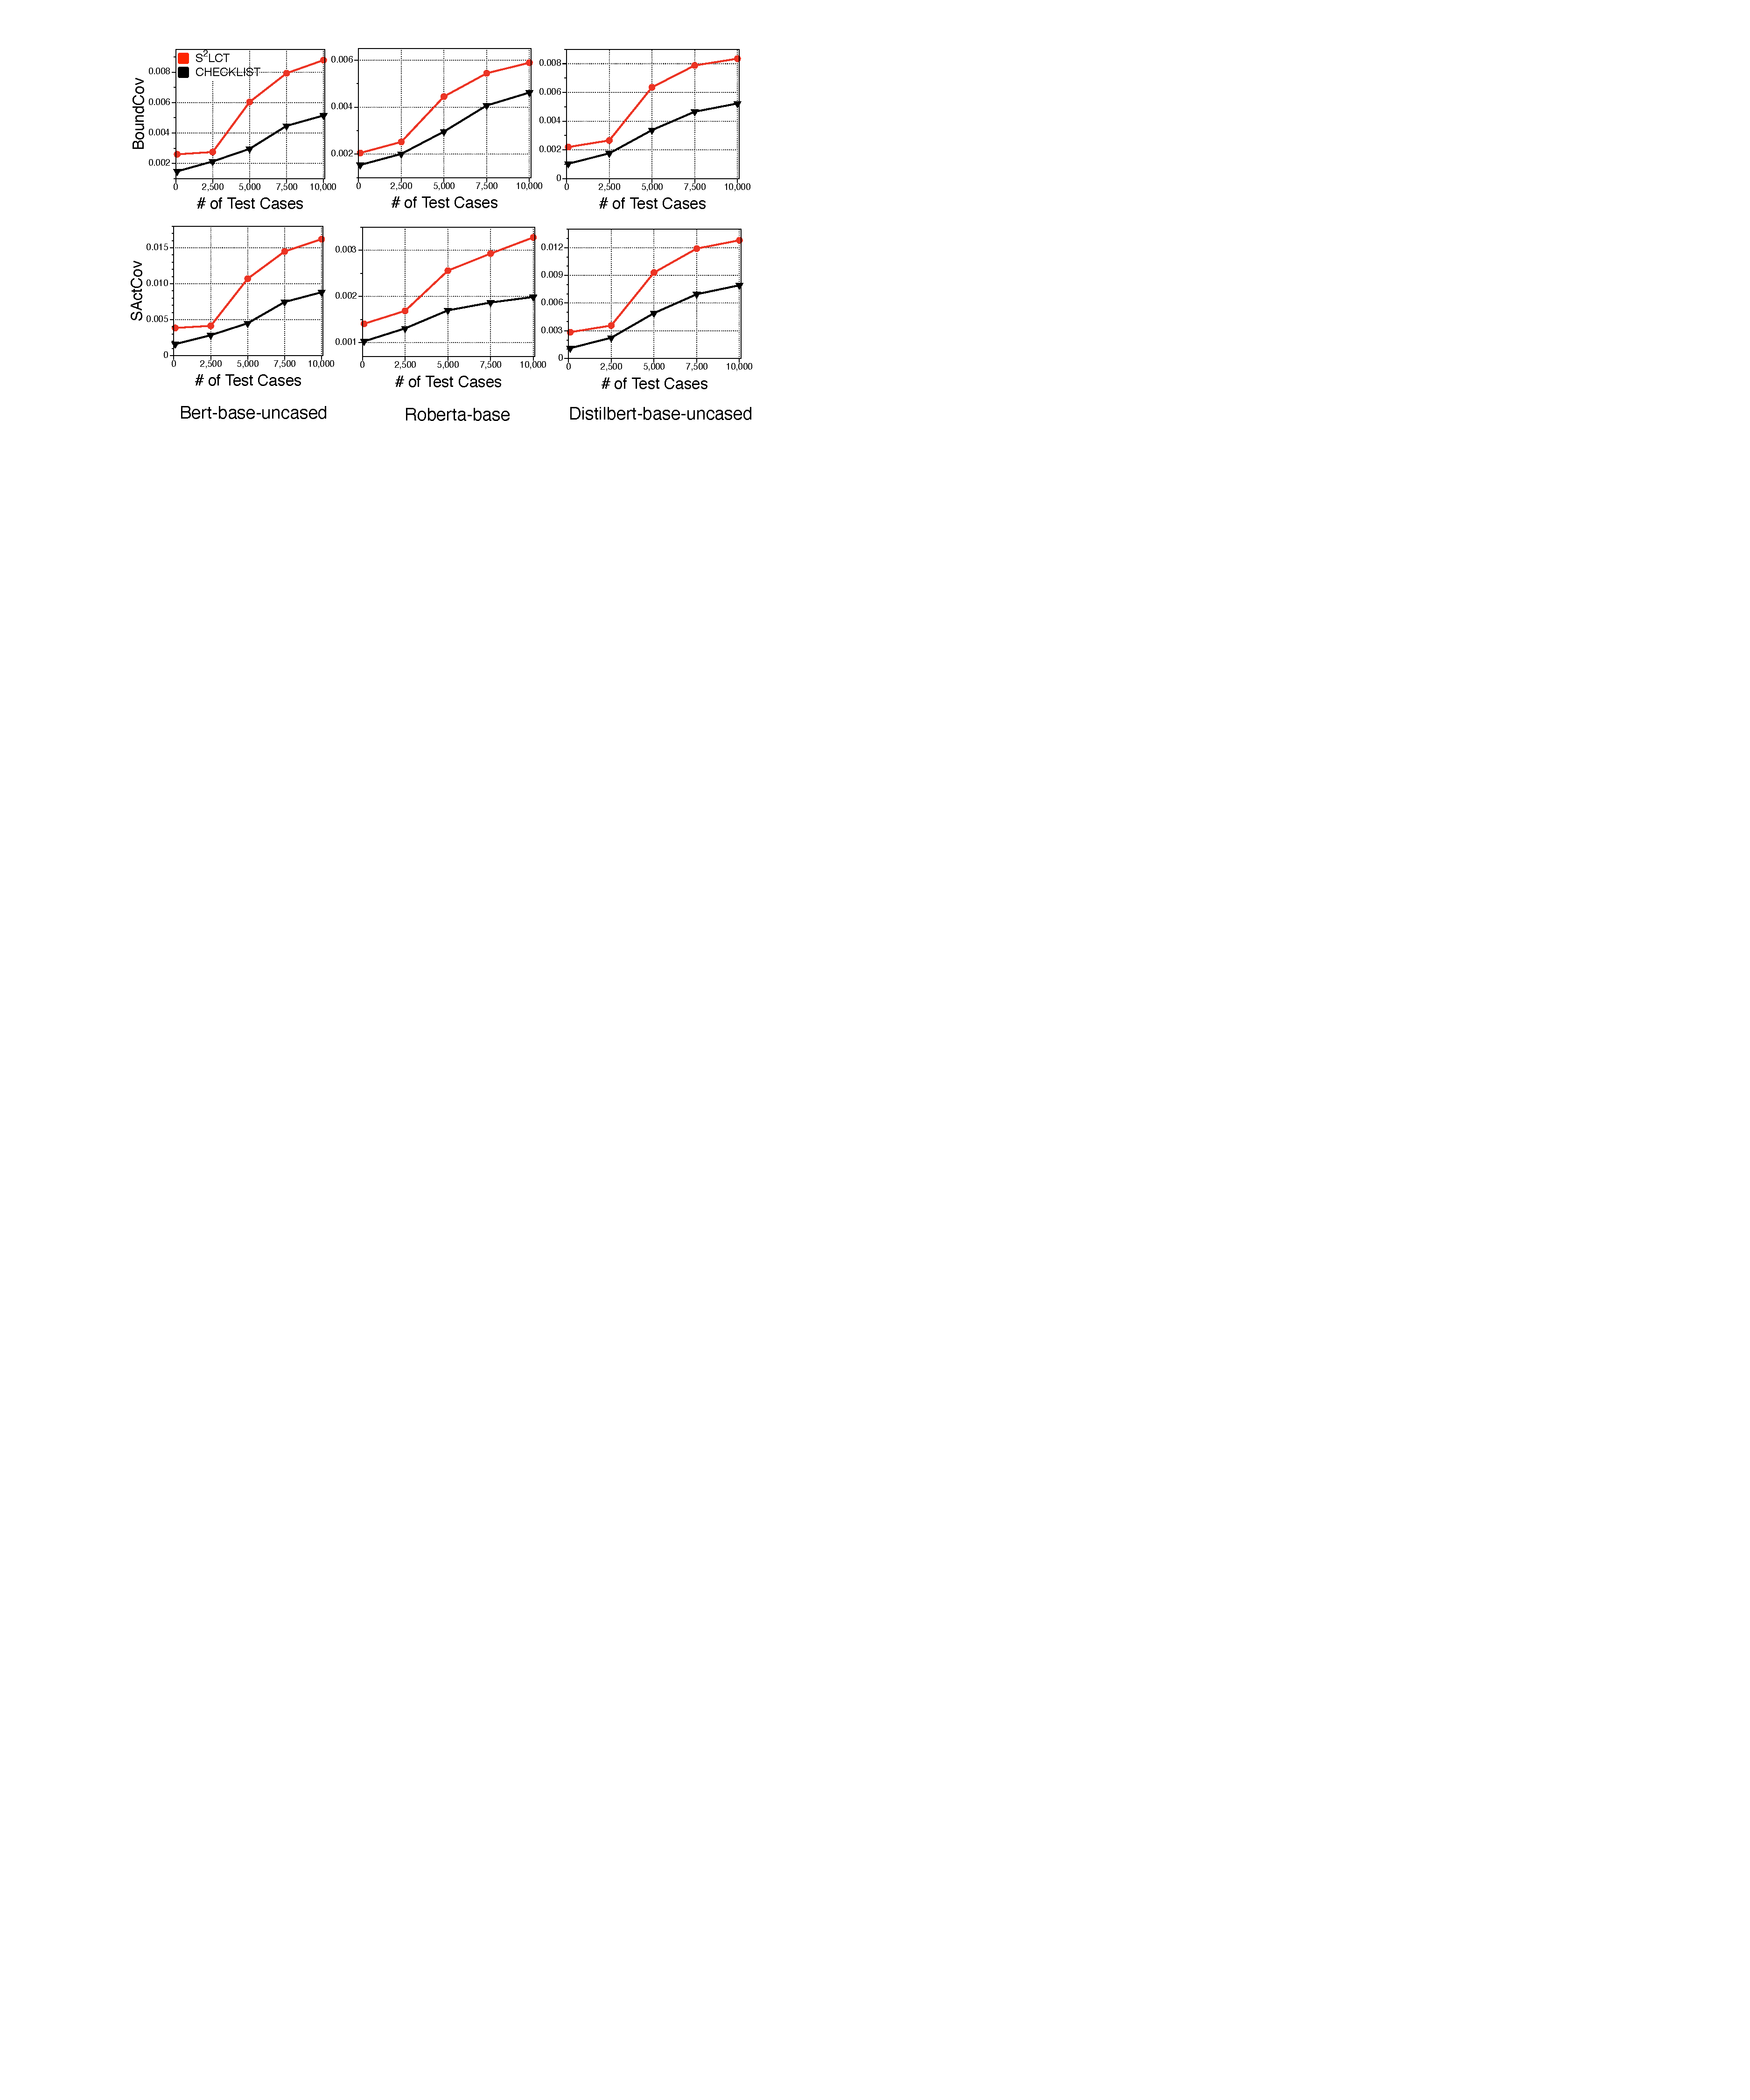
\includegraphics[width=0.5\textwidth]{figs/coverage.pdf}
    \vspace{-4mm}
    \caption{Coverage results of \tool and \Cklst test cases.}
    \label{fig:coverage}
\end{figure}

Next, Figure \ref{fig:coverage} shows the coverage results of \tool and \Cklst test cases. The red line represents \tool coverage and the black line represents \Cklst coverage. Each column in Figure \ref{fig:coverage} represents the results for one NLP model. The first row is the \textit{BoundCov} results and the second row is the \textit{SActCov} results.

We made three observations.
First, for \emph{all} experimental settings (i.e., NLP model and coverage metric), \tool achieves higher coverage than \Cklst. Recall that a higher coverage implies the test cases are more diverse and do not have a similar statistical distribution to the model training data. As a result, a test suite with greater coverage complements the model training data distribution (\ie holdout testing data) better.
For example, for the first NLP model under test, \tool can achieve a higher coverage than \Cklst with only half the number of test cases.
This result confirms that \tool can generate more diverse test cases to complement the holdout dataset for testing NLP models.

Second, as the number of test cases increases, the test suite can achieve better coverage. Such observation is intuitive. However, generating a more extensive test suite is not easy, particularly  for \Cklst, which is a manually template-based approach.

Third, for each NLP model, there is no fixed relationship between \textit{BoundCov} and \textit{SActCov}. In other words, while a test suite may produce higher \textit{BoundCov} for some models, the same test suite may get higher \textit{SActCov} for other NLP models.
Recall that \textit{BoundCov} measures both the upper and lower corner neurons and \textit{SActCov} measures only the upper corner neurons. 
Such observation implies that the upper and lower corner neurons are distributed unevenly, and measuring only one of them is not enough.

\InputWithSpace{tables/manual-study-table}

\subsection{RQ2: Correctness of Sentiment Labels}
Table~\ref{table:ManualStudy} shows results of our manual study. The first column distinguishes the seed and expanded sentences. The number of test cases used for the study is represented in the
second column. The label consistency score defined
in Equation~\ref{metric:srel} is shown in column 3.

We observe that \emph{\tool generates test cases that consistently
  label their sentiment correctly.}  Column 3 shows that the label
consistency scores are 0.83 and 0.84 for the seed and expanded
sentences, respectively.
This means that \tool generates test oracles consistent with
human understanding most of the time. Also, there is
little difference of the scores between the seed and expanded
sentences. This implies that the syntax-based sentence expansion in
\tool preserves the sentiment as its seed.

% \sw{This paragraph is problematic. We are saying the inconsistency is just caused by human, indicating our tool is always correct?} Nevertheless, there exist inconsistency between \tool and manual labels. The causes of inconsistency are twofold. First, complicated sentences have led the participants to
% misunderstand its meaning. Second, phrase in a sentence has
% multiple interpretations of its sentiment. For example, the
% word ``easy'' could be interpreted as both compliment and back-handed
% insult.  
%% \sw{What are
%%   the causes of inconsistency? Looks like the main source of
%%   inconsistency comes from seed generation? Any insights on how it
%%   happened (e.g., issue with original labels, search rules, or
%%   templates?}

\subsection{RQ3: Correctness of Linguistic Capability Categorization}

The \lc relevancy score defined
in Equation~\ref{metric:lcrel} is shown in Column 4 of Table \ref{table:ManualStudy}. The result shows that
\emph{\tool generates test cases that are correctly categorized to the corresponding linguistic capabilities most of the time.}
The \lc relevancy scores for the seed and expanded sentences are both 0.9, achieving high order of agreement with human assessment. The fact that the expanded sentences
generated by \tool also have the same level of \lc
relevancy as the seed sentences shows that the syntax-based sentence expansion retains the linguistic capabilities.


\subsection{RQ4: Use \tool for Understanding Errors}


\begin{figure*}
    \centering
    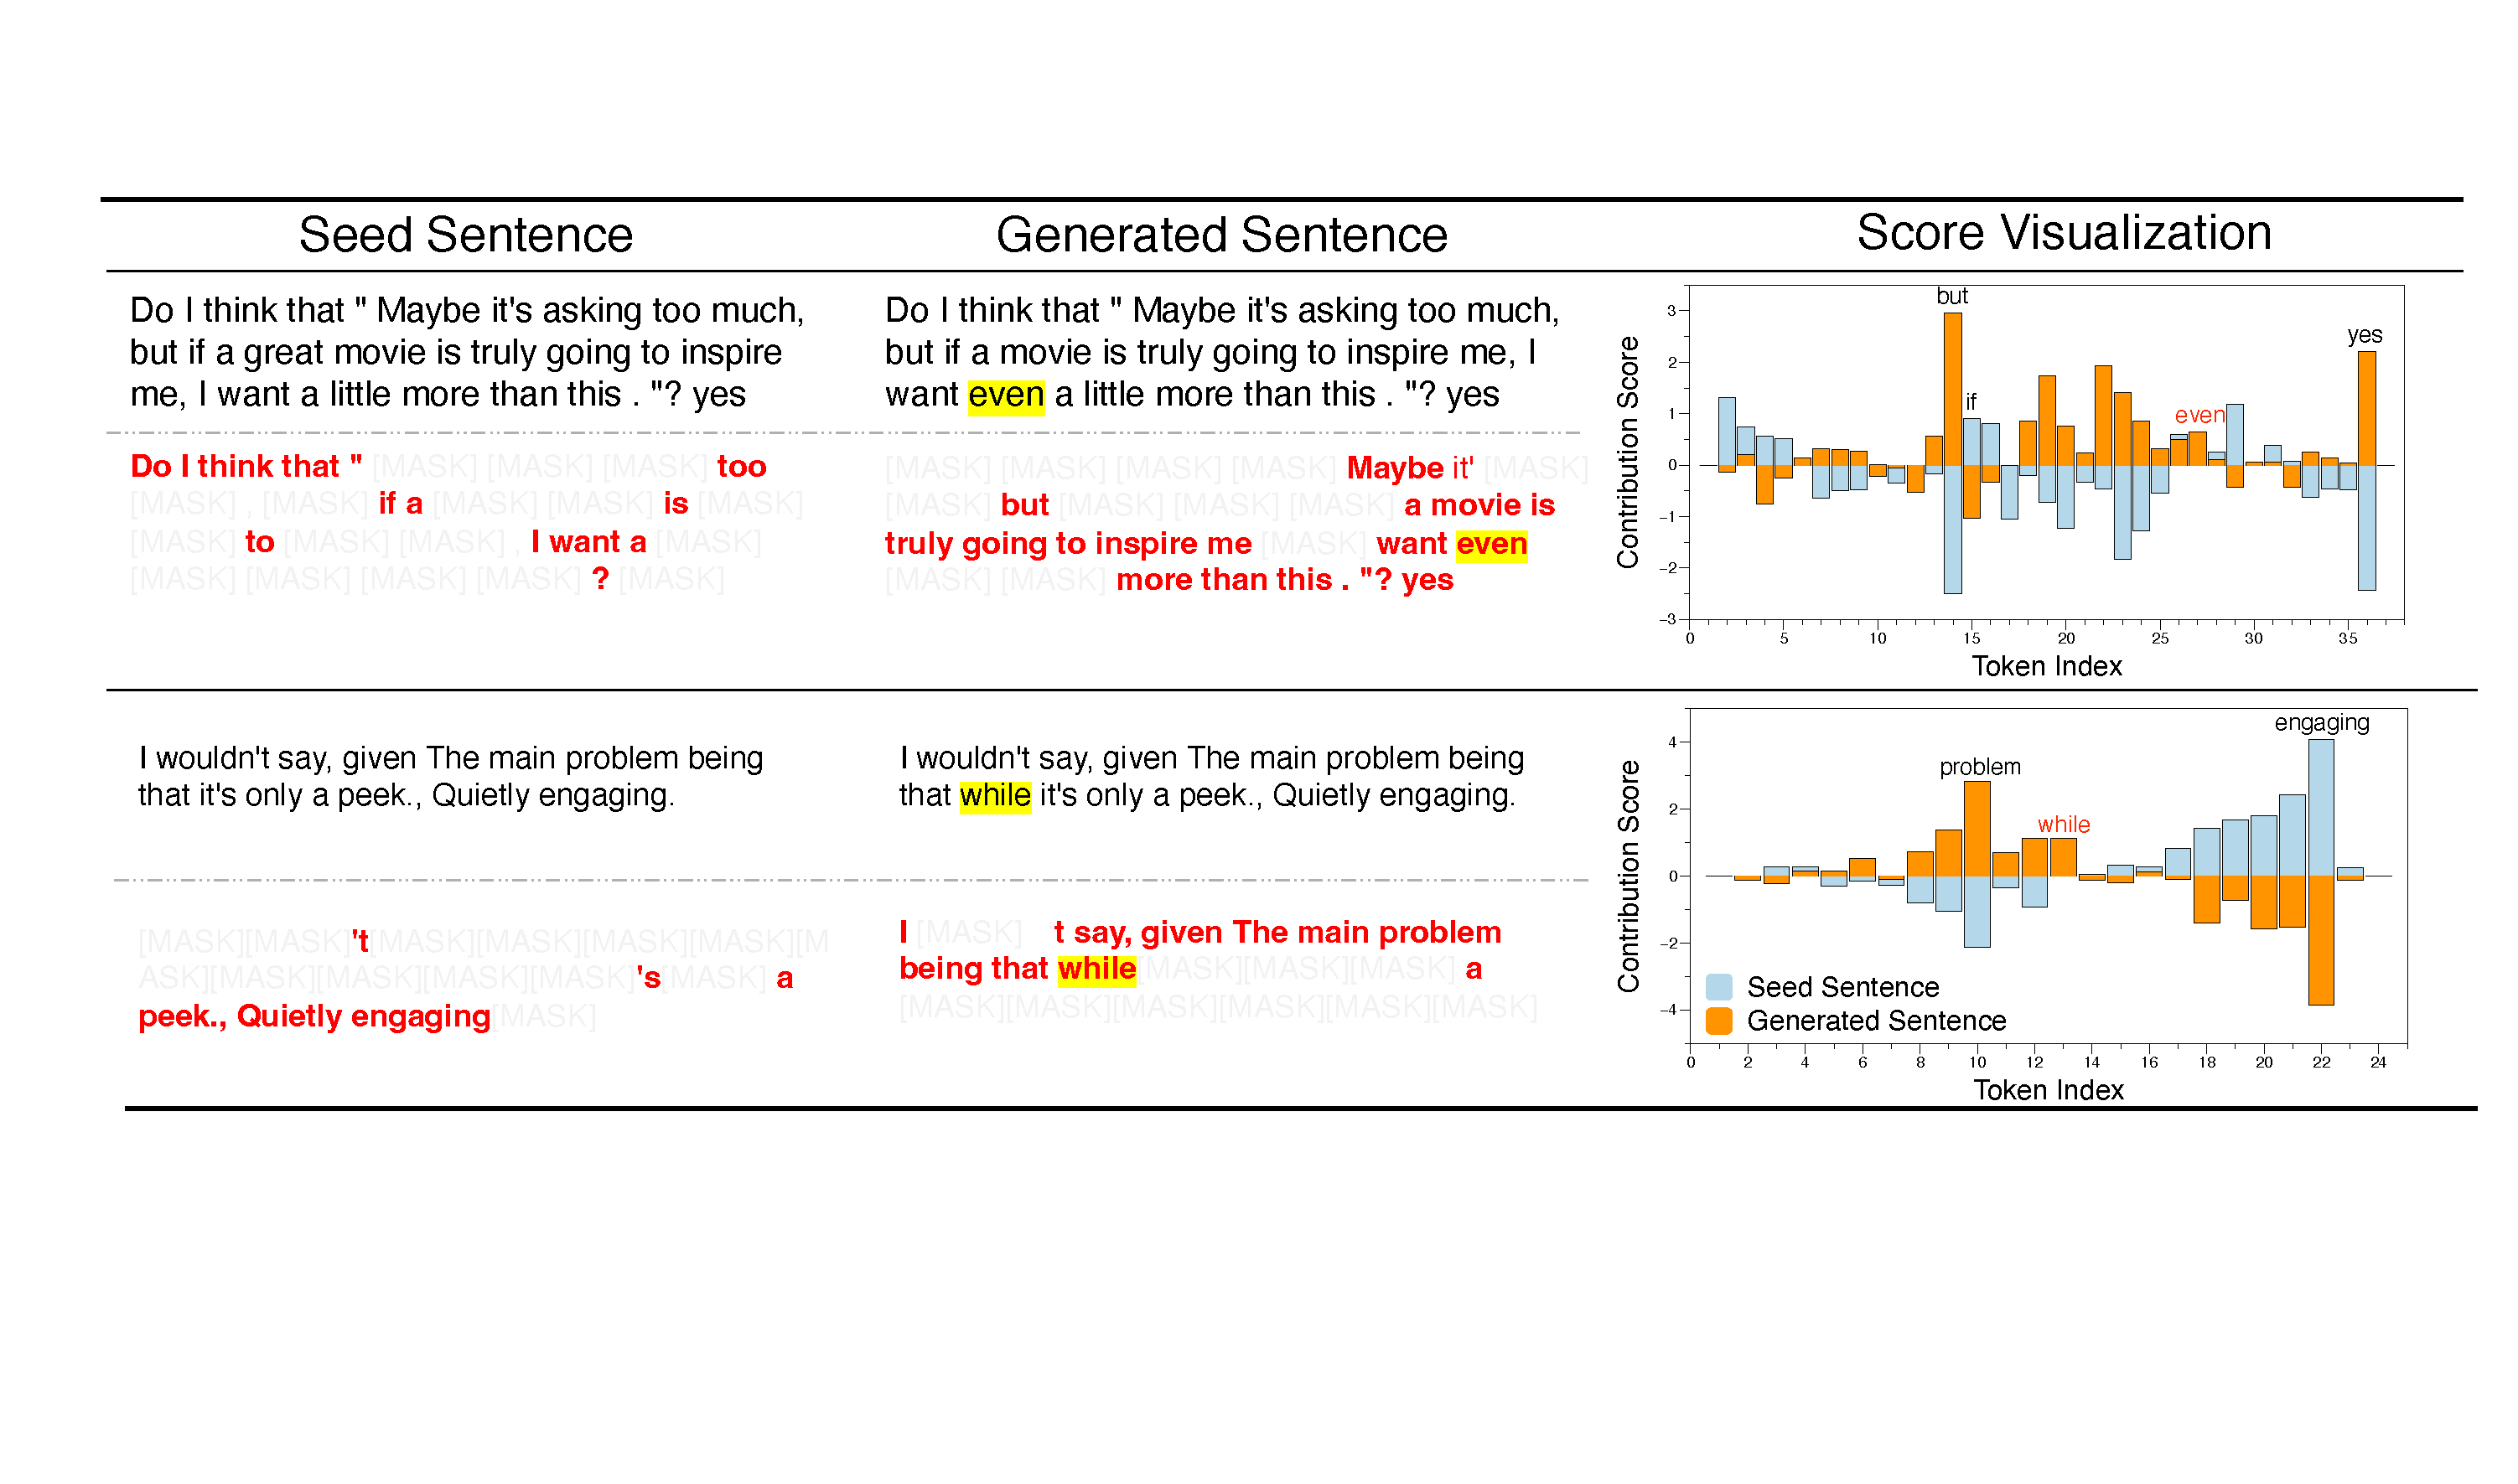
\includegraphics[width=0.99\textwidth]{figs/explain.pdf}
    \vspace{-4mm}
    \caption{Visualization of the buggy reason of two \tool generated test cases.}
    \label{fig:explain}
\end{figure*}


Recall our RQ4 is to generate a template that will dominate the NLP model prediction to assist developers in understanding the false predictions. Figure \ref{fig:explain} shows the generated templates for two randomly selected seed inputs and corresponding generated test inputs.
The first example is to test ``sentiments in (question, yes) form'' (LC9), and the second example is to test ``negative positive with neutral content in the middle''  (LC7).
The first column contains the seed sentence, the second contains the generated sentence, and the third contains thCT  of each token's contribution score. The blue bar indicates thxe score for seed inputs, whereas the orange bar reflects the score f CTor created sentences.
We highlight the mutated token with yellow background and generated templates with red text. 

The results show that after mutating the seed sentence with one token, the token set that dominates the NLP model prediction has changed.
We can trace the root causes to the bias of training data on the \lc under test; as a result, for the \lc under test, the model has a bias towards positive/negative for certain token sequence patterns. For example, \lc 9 has a bias toward the token sequence pattern that includes "maybe .... but ... even... yes". Thus, adding the token "even" to the seed sentence will match one of those biased sequence patterns.
Sentences with s.8gmxuin the training dataset are dominantly positive, thus the models makes the wrong decision on the sentence with ``even'' as positive. 
The visualization of each token's contribution score in the third column also confirms our observation. Once  ``even'' is added, scores of other tokens such as ``but'' and ``yes'' all change from negative to positive.
To fix the issue for LC9, we ne ed to add more training negative samples with the 还 of ``maybe . .. but ... even ... yes''.
%he experimental results in Fig. \ref{fig:explain} illustrate that \tool can help developers to understand the buggy reason of the misclassification go no在,
